% author:   sam tenka
% change:   2022-07-05
% create:   2022-07-05

%==============================================================================
%====  0.  DOCUMENT SETTINGS  ================================================
%==============================================================================

%~~~~~~~~~~~~~~~~~~~~~~~~~~~~~~~~~~~~~~~~~~~~~~~~~~~~~~~~~~~~~~~~~~~~~~~~~~~~~~
%~~~~~~~~~~~~~  0.0. About this Exposition  ~~~~~~~~~~~~~~~~~~~~~~~~~~~~~~~~~~~

%---------------------  0.0.0. page geometry  ---------------------------------
\documentclass[11pt, justified]{tufte-book}
\geometry{
  left           = 0.90in, % left margin
  textwidth      = 4.95in, % main text block
  marginparsep   = 0.15in, % gutter between main text block and margin notes
  marginparwidth = 2.30in, % width of margin notes
                 % 0.20in  % width from margin to edge
}

%---------------------  0.0.1. math packages  ---------------------------------
\newcommand\hmmax{0} % to allow for more fonts 
\newcommand\bmmax{0} % to allow for more fonts
\usepackage{amsmath, amssymb, amsthm, mathtools}
\usepackage{bm}
\usepackage{euler}

\usepackage{array}   % for \newcolumntype macro
\newcolumntype{L}{>{$}l<{$}} % math-mode version of "l" column type
\newcolumntype{C}{>{$}c<{$}} % math-mode version of "c" column type
\newcolumntype{R}{>{$}r<{$}} % math-mode version of "r" column type

%---------------------  0.0.2. graphics packages  -----------------------------
\usepackage{graphicx, xcolor}
\usepackage{float, capt-of}

%---------------------  0.0.3. packages for fancy text  -----------------------
\usepackage{enumitem}\setlist{nosep}
\usepackage{listings}
\usepackage{xstring}
\usepackage{fontawesome5}

%---------------------  0.043. colors  ----------------------------------------
\definecolor{mblu}{rgb}{0.05, 0.35, 0.70} \newcommand{\blu}{\color{mblu}}
\definecolor{mbre}{rgb}{0.30, 0.45, 0.60} \newcommand{\bre}{\color{mbre}}
\definecolor{mbro}{rgb}{0.60, 0.05, 0.05} \newcommand{\bro}{\color{mbro}}
\definecolor{mcya}{rgb}{0.10, 0.45, 0.45} \newcommand{\cya}{\color{mcya}}
\definecolor{mgre}{rgb}{0.55, 0.55, 0.50} \newcommand{\gre}{\color{mgre}}
\definecolor{mgrn}{rgb}{0.15, 0.65, 0.05} \newcommand{\grn}{\color{mgrn}}
\definecolor{mred}{rgb}{0.90, 0.05, 0.05} \newcommand{\red}{\color{mred}}

%~~~~~~~~~~~~~~~~~~~~~~~~~~~~~~~~~~~~~~~~~~~~~~~~~~~~~~~~~~~~~~~~~~~~~~~~~~~~~~
%~~~~~~~~~~~~~  0.1. Headers and References  ~~~~~~~~~~~~~~~~~~~~~~~~~~~~~~~~~~

%---------------------  0.1.0. intra-document references  ---------------------
\newcommand{\offour}[1]{
    {\tiny \raisebox{0.04cm}{\scalebox{0.9}{$\substack{
        \IfSubStr{#1}{0}{{\blacksquare}}{\square}   
        \IfSubStr{#1}{1}{{\blacksquare}}{\square} \\ 
        \IfSubStr{#1}{2}{{\blacksquare}}{\square}   
        \IfSubStr{#1}{3}{{\blacksquare}}{\square}   
    }$}}}%
}

\newcommand{\offourline}[1]{
    {\tiny \raisebox{0.04cm}{\scalebox{0.9}{$\substack{
        \IfSubStr{#1}{0}{{\blacksquare}}{\square}   
        \IfSubStr{#1}{1}{{\blacksquare}}{\square}
        \IfSubStr{#1}{2}{{\blacksquare}}{\square}   
        \IfSubStr{#1}{3}{{\blacksquare}}{\square}   
    }$}}}%
}
\newcommand{\notesam}[1]{{\blu \textsf{#1}}}
\newcommand{\attn}[1]{{\bro \textsf{#1}}}
\newcommand{\attnsam}[1]{{\red \textsf{#1}}}

\newcommand{\blarr}{\hspace{-0.15cm}${\bro \leftarrow}\,$}
\newcommand{\bcirc}{${\bro ^\circ}$}

%---------------------  0.1.1. table of contents helpers  ---------------------
\newcommand{\phdot}{\phantom{.}}

%---------------------  0.1.2. section headers  -------------------------------
\newcommand{\samtitle} [1]{
  \par\noindent{\Huge \sf \blu #1}
  \vspace{0.4cm}
}

\newcommand{\samquote} [2]{
    \marginnote[-0.4cm]{\begin{flushright}
    \scriptsize
        \gre {\it #1} \\ --- #2
    \end{flushright}}
}

\newcommand{\samsection} [1]{
  \vspace{0.5cm}
  \par\noindent{\LARGE \sf \blu #1}
  \vspace{0.1cm}\par
}

\newcommand{\samsubsection}[1]{
  \vspace{0.3cm}
  \par\noindent{\Large \sf \bre #1}
  \vspace{0.1cm}\par
}

\newcommand{\samsubsubsection}[1]{
   \vspace{0.1cm}
   \par\noindent{\hspace{-2cm}\normalsize \sc \gre #1} ---
}

%---------------------  0.1.3. clear the bibliography's header  ---------------
\usepackage{etoolbox}
\patchcmd{\thebibliography}{\section*{\refname}}{}{}{}

%~~~~~~~~~~~~~~~~~~~~~~~~~~~~~~~~~~~~~~~~~~~~~~~~~~~~~~~~~~~~~~~~~~~~~~~~~~~~~~
%~~~~~~~~~~~~~  0.2. Math Symbols and Blocks  ~~~~~~~~~~~~~~~~~~~~~~~~~~~~~~~~~

%---------------------  0.2.0. general math operators  ------------------------
\newcommand{\scirc}{\mathrel{\mathsmaller{\mathsmaller{\mathsmaller{\circ}}}}}
\newcommand{\cmop}[2]{{(#1\!\to\!#2)}}
\newcommand{\pr}{\prime}

%---------------------  0.2.1. probability symbols  ---------------------------
\newcommand{\KL}{\text{KL}}
\newcommand{\EN}{\text{H}}
\newcommand{\note}[1]{{\blu \textsf{#1}}}

%---------------------  0.2.2. losses averaged in various ways  ---------------
\newcommand{\Ein}  {\text{trn}_{\sS}}
\newcommand{\Einb} {\text{trn}_{\check\sS}}
\newcommand{\Einc} {\text{trn}_{\sS\sqcup \check\sS}}
\newcommand{\Egap} {\text{gap}_{\sS}}
\newcommand{\Eout} {\text{tst}}

%---------------------  0.2.3. double-struck and caligraphic upper letters  ---
\newcommand{\Aa}{\mathbb{A}}\newcommand{\aA}{\mathcal{A}}
\newcommand{\Bb}{\mathbb{B}}\newcommand{\bB}{\mathcal{B}}
\newcommand{\Cc}{\mathbb{C}}\newcommand{\cC}{\mathcal{C}}
\newcommand{\Dd}{\mathbb{D}}\newcommand{\dD}{\mathcal{D}}
\newcommand{\Ee}{\mathbb{E}}\newcommand{\eE}{\mathcal{E}}
\newcommand{\Ff}{\mathbb{F}}\newcommand{\fF}{\mathcal{F}}
\newcommand{\Gg}{\mathbb{G}}\newcommand{\gG}{\mathcal{G}}
\newcommand{\Hh}{\mathbb{H}}\newcommand{\hH}{\mathcal{H}}
\newcommand{\Ii}{\mathbb{I}}\newcommand{\iI}{\mathcal{I}}
\newcommand{\Jj}{\mathbb{J}}\newcommand{\jJ}{\mathcal{J}}
\newcommand{\Kk}{\mathbb{K}}\newcommand{\kK}{\mathcal{K}}
\newcommand{\Ll}{\mathbb{L}}\newcommand{\lL}{\mathcal{L}}
\newcommand{\Mm}{\mathbb{M}}\newcommand{\mM}{\mathcal{M}}
\newcommand{\Nn}{\mathbb{N}}\newcommand{\nN}{\mathcal{N}}
\newcommand{\Oo}{\mathbb{O}}\newcommand{\oO}{\mathcal{O}}
\newcommand{\Pp}{\mathbb{P}}\newcommand{\pP}{\mathcal{P}}
\newcommand{\Qq}{\mathbb{Q}}\newcommand{\qQ}{\mathcal{Q}}
\newcommand{\Rr}{\mathbb{R}}\newcommand{\rR}{\mathcal{R}}
\newcommand{\Ss}{\mathbb{S}}\newcommand{\sS}{\mathcal{S}}
\newcommand{\Tt}{\mathbb{T}}\newcommand{\tT}{\mathcal{T}}
\newcommand{\Uu}{\mathbb{U}}\newcommand{\uU}{\mathcal{U}}
\newcommand{\Vv}{\mathbb{V}}\newcommand{\vV}{\mathcal{V}}
\newcommand{\Ww}{\mathbb{W}}\newcommand{\wW}{\mathcal{W}}
\newcommand{\Xx}{\mathbb{X}}\newcommand{\xX}{\mathcal{X}}
\newcommand{\Yy}{\mathbb{Y}}\newcommand{\yY}{\mathcal{Y}}
\newcommand{\Zz}{\mathbb{Z}}\newcommand{\zZ}{\mathcal{Z}}

%---------------------  0.2.4. sans serif and frak lower letters  -------------
\newcommand{\sfa}{\mathsf{a}}\newcommand{\fra}{\mathcal{a}}
\newcommand{\sfb}{\mathsf{b}}\newcommand{\frb}{\mathcal{b}}
\newcommand{\sfc}{\mathsf{c}}\newcommand{\frc}{\mathcal{c}}
\newcommand{\sfd}{\mathsf{d}}\newcommand{\frd}{\mathcal{d}}
\newcommand{\sfe}{\mathsf{e}}\newcommand{\fre}{\mathcal{e}}
\newcommand{\sff}{\mathsf{f}}\newcommand{\frf}{\mathcal{f}}
\newcommand{\sfg}{\mathsf{g}}\newcommand{\frg}{\mathcal{g}}
\newcommand{\sfh}{\mathsf{h}}\newcommand{\frh}{\mathcal{h}}
\newcommand{\sfi}{\mathsf{i}}\newcommand{\fri}{\mathcal{i}}
\newcommand{\sfj}{\mathsf{j}}\newcommand{\frj}{\mathcal{j}}
\newcommand{\sfk}{\mathsf{k}}\newcommand{\frk}{\mathcal{k}}
\newcommand{\sfl}{\mathsf{l}}\newcommand{\frl}{\mathcal{l}}
\newcommand{\sfm}{\mathsf{m}}\newcommand{\frm}{\mathcal{m}}
\newcommand{\sfn}{\mathsf{n}}\newcommand{\frn}{\mathcal{n}}
\newcommand{\sfo}{\mathsf{o}}\newcommand{\fro}{\mathcal{o}}
\newcommand{\sfp}{\mathsf{p}}\newcommand{\frp}{\mathcal{p}}
\newcommand{\sfq}{\mathsf{q}}\newcommand{\frq}{\mathcal{q}}
\newcommand{\sfr}{\mathsf{r}}\newcommand{\frr}{\mathcal{r}}
\newcommand{\sfs}{\mathsf{s}}\newcommand{\frs}{\mathcal{s}}
\newcommand{\sft}{\mathsf{t}}\newcommand{\frt}{\mathcal{t}}
\newcommand{\sfu}{\mathsf{u}}\newcommand{\fru}{\mathcal{u}}
\newcommand{\sfv}{\mathsf{v}}\newcommand{\frv}{\mathcal{v}}
\newcommand{\sfw}{\mathsf{w}}\newcommand{\frw}{\mathcal{w}}
\newcommand{\sfx}{\mathsf{x}}\newcommand{\frx}{\mathcal{x}}
\newcommand{\sfy}{\mathsf{y}}\newcommand{\fry}{\mathcal{y}}
\newcommand{\sfz}{\mathsf{z}}\newcommand{\frz}{\mathcal{z}}

%---------------------  0.2.5. math environments  -----------------------------
\newtheorem*{qst}{Question}
\newtheorem*{thm}{Theorem}
\newtheorem*{lem}{Lemma}
% ...
\theoremstyle{definition}
\newtheorem*{dfn}{Definition}

%==============================================================================
%=====  1.  DOCUMENT PROPER  ==================================================
%==============================================================================

\begin{document}

  %\newcommand{}{\textsc{Philip,  Mariana, Mawuko}}
  %\newcommand{ }{\textsc{James,   Bereket, Amadeo}}
  %%
  %\newcommand{}   {\textsc{Philip,  James}}
  %\newcommand{}   {\textsc{Mariana, Bereket}}
  %\newcommand{}   {\textsc{Mawuko,  Amadeo}}
  %
  %\newcommand{\exercise}[2]{\par\noindent\attn{Exercise} (#1): \emph{#2}}
  \newcommand{\exercise}[2]{\par\noindent\attn{Exercise}: \emph{#2}}
  %\newcommand{\exercise}[2]{\marginnote{\attn{Exercise} (#1): \emph{#2}}}

%~~~~~~~~~~~~~~~~~~~~~~~~~~~~~~~~~~~~~~~~~~~~~~~~~~~~~~~~~~~~~~~~~~~~~~~~~~~~~~
%~~~~~~~~~~~~~  1.0. front matter  ~~~~~~~~~~~~~~~~~~~~~~~~~~~~~~~~~~~~~~~~~~~~

  \samtitle{rec 07:
            ideas in neural architecture}

  \noindent
    Let's discuss neural networks design choices.  By today's end, we'll be
    able to:\marginnote{%
    Our rough schedule is:
    \begin{description}
        \item[\hspace{0.25cm}] \emph{19:30} width and depth
        \item[\hspace{0.25cm}] \emph{19:45} initialization, expressivity
        \item[\hspace{0.25cm}] \emph{20:00} `to build a tool, use it'
        \item[\hspace{0.25cm}] \emph{20:15} latent representations 
        \item[\hspace{0.25cm}] \emph{20:30} symmetries
        \item[\hspace{0.25cm}] \emph{20:45} rnns: `derivation', backprop practice 
        \item[\hspace{0.25cm}] \emph{21:00} 
    \end{description}
    }
    \begin{description}
        \item[\hspace{1cm}] \emph{tailor} a neural network to a task's inherent
                            dependencies
        \item[\hspace{1cm}] \emph{exploit} a task's symmetries to improve
                            generalization.
        %\item[\hspace{1cm}] \emph{train} an RNN to do basic sentiment analysis.
        \item[\hspace{1cm}] \emph{explain} the assumptions behind each design choice
            leading to RNNs 
        %\item[\hspace{1cm}] \emph{initialize} weights to avoid stalled training 
            % TODO: also discuss bottlenecks / gradient boosts?
    \end{description}
    As always, \attn{please ask questions} at any time, including by
    interrupting me!

  \samsection{C. automatic featurization, continued}
    %\samsubsection{new features from old}
    %\samsubsection{fitting features to data}
    %\samsubsection{dynamics of shallow net learning}

    %

    \samsubsection{basic architecture: width and depth}
      \samsubsubsection{last time: width}\vspace{-0.5cm}
        \begin{figure}[h]
          \centering
              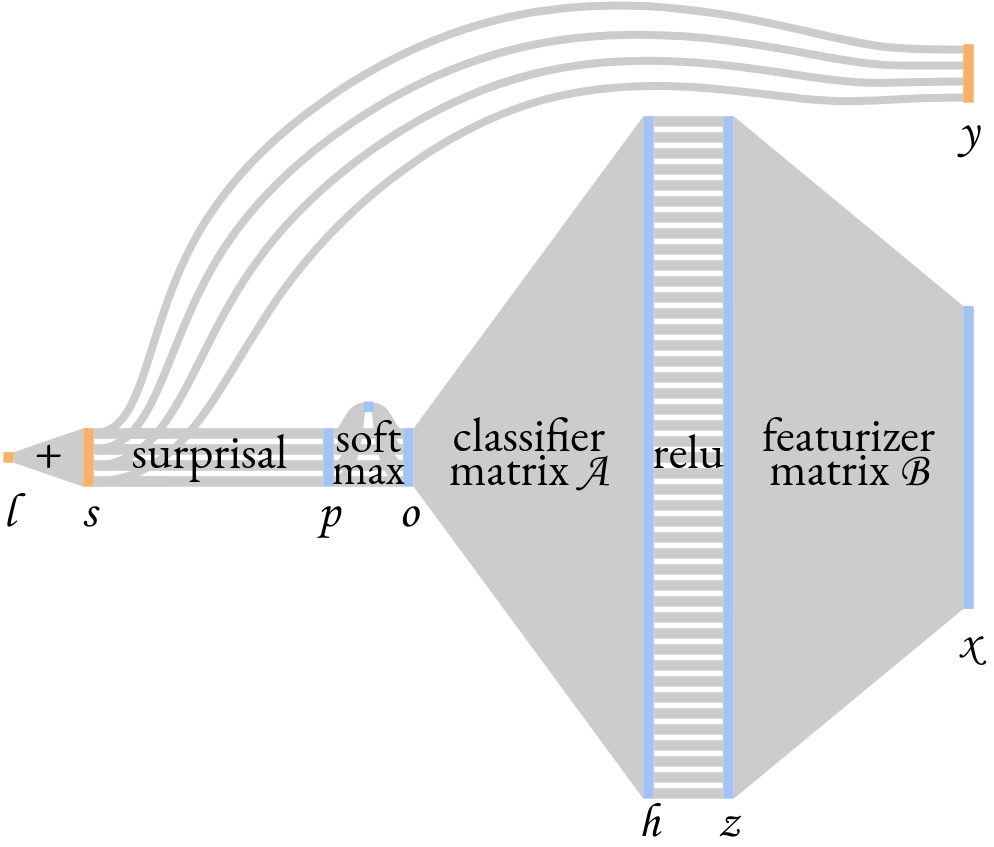
\includegraphics[width=0.500\textwidth]{shallow}
          \caption{%
            \textbf{Shallow neural nets.} Data flows right to left via {\gre
            gray} transforms.  We use the {\blu blue} quantities to predict;
            the {\color{orange} orange}, to train.  Thin vertical
            strips depict vectors; small squares, scalars.  
            %
            We train the net to maximize data likelihood per its softmax
            predictions:\vspace{-0.1cm}
            %
            $$
                \ell = \textstyle\sum_k s_k 
                \quad
                s_k = y_k \log(1/p_k)
            $$
            \vspace{-0.4cm}
            $$
                p_k = \exp(o_k) /\!\textstyle\sum_{\tilde k} \exp(o_{\tilde k})
            $$
            %
            The decision function $o$ is a linear combination of features $h$
            nonlinearly transformed from $x$:\vspace{-0.1cm}
            $$
                o_k = \textstyle\sum_{j} A_{kj} h_j 
            $$
            Each ``\textbf{hidden activation}'' or ``\textbf{learned feature}''
            $h_j$ measures tresspass past a linear boundary determined by a
            vector $B_j$:\vspace{-0.1cm}
            $$
                h_j = \text{relu}(z_j) = \max(0,z_j)
                \quad
                z_j = \textstyle\sum_{i} B_{ji} x_i 
            $$
          }
        \end{figure}%
      \samsubsubsection{today: also depth}\vspace{-0.5cm}
        \begin{figure}[h]
          \centering
              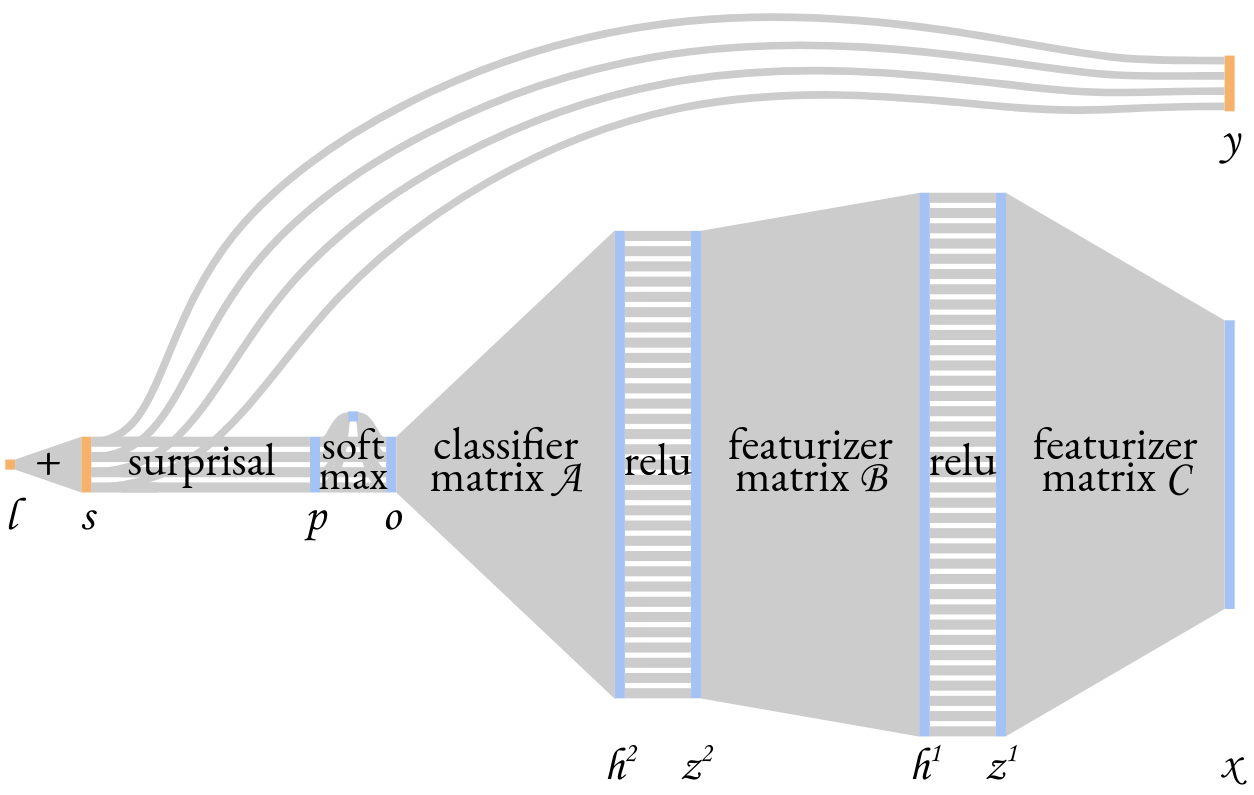
\includegraphics[width=0.700\textwidth]{deep}
          \caption{%
            \textbf{A deeper neural net.} As before, data flows right to left
            via {\gre gray} transforms.
            %
            We train the net to maximize data likelihood per its softmax
            predictions and the decision function $o$ is a linear combination
            of features $h^2$ nonlinearly transformed from $x$.
            %
            However, that nonlinear transform is now less direct: we transform
            $x$ to a first layer $h^1$ of hidden features and then to $h^2$.
            Explicitly:\vspace{-0.1cm}
            $$
                h^2_j = \text{relu}(z^2_j) 
                \quad
                z^2_j = \textstyle\sum_{i} B_{ji} h^1_i 
            $$
            and\vspace{-0.1cm}
            $$
                h^1_j = \text{relu}(z^2_j)
                \quad
                z^1_j = \textstyle\sum_{i} C_{ji} x_i 
            $$
            We may regard $x$ as $h^0$ and $o$ as $z^3$ if we wish.
            We say this net has a \textbf{depth} of
            \textbf{three weight layers} or of \textbf{two hidden layers}. 
          }
        \end{figure}

        The next three questions consider classifying
        raw dimension-$784$ inputs into $10$ classes.  We'll answer in terms of
        the dimensions (one number for the shallow net; two for the deeper net)
        of the hidden layers.
        %
        \exercise{}{How many parameters does the shallow net have, ignoring
                    bias terms?}
        %
        \exercise{}{How many parameters does the deeper net have, ignoring 
                    bias terms?}
        %
        \exercise{}{How about if we allow bias terms for each weight layer?}

        \newpage
      \samsubsubsection{initialization}
        In the next three questions, we initialize all weights to zero.  We're
        doing binary classification without weight regularization.
        %
        \exercise{}{What is the training loss at initialization?}
        %
        \exercise{}{What is the loss gradient at initialization?}
        %
        \exercise{}{What is the testing loss after a thousand SGD
        updates?}

        Due to the pathology\bcirc \marginnote{%
          \blarr The nonconvexity of learning --- as evidenced by permutation
          symmetry of hidden features in the model --- allows this pathology.  
        }
        uncovered in the above exercises, we like to \emph{randomly} initialize
        our weights.
        %
        What distribution should we use?
        %
        In what follows, we focus on the input-most layer defined on an input
        vector $x$ by $h^1_j = \text{relu}\left(\sum_i C_{ji} x_i \right)$.  We
        assume that $D^1 \times D^0$ many matrix elements $C_{ji}$s are chosen
        independently according to some centered distribution with expected
        absolute value $s$.
        %%\marginnote{%
        %%    \textbf{Technicalities}.  Let's assume a light-tailed distribution
        %%    such as a normal distribution.  Note that the product of two
        %%    independent normals with variances
        %%    has a heavier, $\chi^2$ kind of tail.  Say the two normals have
        %%    (mean, variance) $(0,v)$ and $(m,w)$, respectively.  Then the product
        %%    has mean $0$ and variance 
        %%    Still, the latter has zero mean and variance the product of the
        %%    variances.
        %%}
        %
        \exercise{}{If each $|x_i| \approx 1$ then each $|z^1_j| \approx$
        what?}
        %
        \exercise{}{If each $|x_i| \approx 1$ then each $|h^1_j| \approx$
        what?}
        %
        \exercise{}{If each $|x_i| \approx 1$ and each $|\partial \ell/\partial
        h_j| \approx 1$ then each $|\partial \ell/\partial x_i| \approx$ what?}

        So for calibrated forward propagation, we might initialize each $C_{ji}$
        to have scale roughly $\sqrt{2/D^0}$.\bcirc\marginnote{%
            \blarr Don't pay much heed to the constant factor $2$.
        }
        %
        For calibrated backward propagation, we might initialize each $C_{ji}$
        to have scale roughly $\sqrt{2/D^1}$.
        %
        We often use a compromise:\bcirc\marginnote{%
            \blarr This formula is named after \textbf{Glorot, Bengio, Xavier},
            and probably others.  Don't pay much heed to the constant factor
            $4$. 
        }
        $$
            |C_{ji}| \approx \sqrt{\frac{4}{D^1+D^0}}
        $$
        For example, we can initialize by sampling $C_{ji}$ from a centered
        normal with variance $4/(D^1+D^0)$.  The tension between the forward
        and backward scales is least\bcirc when $D^1 \approx D^0$.\marginnote{%
          \blarr This is a weak
          reason to favor gradual rather than abrupt changes in dimension across
          a neural network.  It's a weak reason because one could also counter
          this tension by using different learning rates for each layer.
          %
          In practice, adaptive methods such as ADAM automatically do the
        latter.
        }

      %\samsubsubsection{learning rates}
      %  \exercise{}{If each $|x_i| \approx 1$ and each $|\partial \ell/\partial
      %  h_j| \approx 1$ then each $|\partial \ell/\partial C_{ji}| \approx$
      %  what?}
      %  %

      %\newpage
      \newcommand{\decade}[2]{
          \includegraphics[width=0.099\textwidth]{#1-#20}%
          \includegraphics[width=0.099\textwidth]{#1-#21}%
          \includegraphics[width=0.099\textwidth]{#1-#22}%
          \includegraphics[width=0.099\textwidth]{#1-#23}%
          \includegraphics[width=0.099\textwidth]{#1-#24}%
          \includegraphics[width=0.099\textwidth]{#1-#25}%
          \includegraphics[width=0.099\textwidth]{#1-#26}%
          \includegraphics[width=0.099\textwidth]{#1-#27}%
          \includegraphics[width=0.099\textwidth]{#1-#28}%
          \includegraphics[width=0.099\textwidth]{#1-#29}\\%
      }
      \samsubsubsection{expressivity}
        Both \textbf{wider} and \textbf{deeper} neural nets (more
        hidden features per hidden layer; more hidden layers) have more supple
        decision boundaries than smaller neural nets.  We can ``spend''
        parameters on increased width or increased depth: both add complexity,
        much like increasing the regularization weakness $C=1/\lambda$.
        %
        Intuitively, increasing width is like enriching a child's vocabulary
        while increasing depth is like enriching a child's grammar.  The
        question \emph{Would the cow have helped its kin had not that act been
        what we loved?} consists of simple, one-syllable words but expresses a
        pretty sophisticated idea.

        %It's more realistic to consider high dimensional inputs.
        %
        So let's
          consider a neural network $\mathcal{N}$ with one hidden layer and with
          layer dimensions $(1 \leftarrow 30 \leftarrow 100)$.
          This has roughly $3000$ many parameters.
          %
          By contrast, we could try a network $\mathcal{N}^\pr$ with two hidden layers
          and with layer dimensions $(1 \leftarrow 25 \leftarrow 25 \leftarrow
          100)$.  This also has roughly $3100$ many parameters.
          %
        Which of these decision boundaries can $\mathcal{N}^\pr$ approximate
        much better than $\mathcal{N}$?
        \exercise{}{%
            ...recognizing whether a given $10\times 10$ handwritten ASCII
            character (dark ink on light paper) belongs to the set
            \texttt{0123456789}
            %\texttt{)!@\#\$\%\textasciicircum\&*(}
            %\texttt{ABCDEFGHIJKLM}
            %\texttt{NOPQRSTUVWXYZ}
            %\texttt{abcdefghijklm}
            %\texttt{nopqrstuvwxyz}
            %of standard english characters.
            of standard arabic numerals.
        }
        \exercise{}{%
            ...recognizing whether a given $10\times 10$ bit matrix has
            all rows the same.
        }
        \exercise{}{%
            ...recognizing whether a given $10\times 10$ bit matrix has no 
            two rows the same.
        }
        \exercise{}{%
            ...recognizing whether the input lies within the $100$-dimensional 
            unit ball.
        }

        The above four exercises are written pretty vaguely.  They're just to 
        get us thinking about the geometry of depth.  Exam questions will of
        course be dramatically more precisely posed.

        %
        \newpage
        The following unfairly difficult exercise invites us to consider how
        depth and width affect expressivity.  Unlike the previous exercise, it
        fails to illustrate typical behaviors visible only in high dimensions.

        \exercise{}{(Unfair but educational).  The following four collections
        of images show decision boundaries from randomly initializations of
        four architectures.  The hidden dimensions are $(4), (64), (4,64),
        (64,4)$.  Match architectures to collections.}
        \begin{figure}[h]
          \centering%
            \decade{example-shallow/sketch-2-004}{00}%
            \decade{example-shallow/sketch-2-004}{01}%
            %
            ~\\
            %
            \decade{example-shallow/sketch-2-064}{00}%
            \decade{example-shallow/sketch-2-064}{01}%
            %
            ~\\
            %
            \decade{example-shallow/sketch-3-064-004}{00}%
            \decade{example-shallow/sketch-3-064-004}{01}%
            %
            ~\\
            %
            \decade{example-shallow/sketch-3-004-064}{00}%
            \decade{example-shallow/sketch-3-004-064}{01}%
          \caption{%
              \textbf{Four collections of decision boundaries}.  Each
              collection shows boundaries for twenty random initializations of
              one of four architecture.  Each plot shows ten by ten unit
              squares with the origin at center.
            %
            %
            \textbf{Top rows}:
            decision boundaries are jagged polygons with edges long and angles moderate. 
            The boundaries show almost no oscillation in their direction of curvature:
            counterclockwise turns are never quickly followed by clockwise turns. 
            The displayed plane tends to be cut into one or two pieces. 
            %
            \textbf{Center top rows}:
            decision boundaries are smooth curves with edges short and angles small. 
            The boundaries show little oscillation in their direction of
            curvature: counterclockwise turns are usually not quickly followed
            by clockwise turns. 
            The displayed plane tends to be cut into one or two pieces. 
            %
            \textbf{Center bottom rows}:
            decision boundaries are jagged curves with edges short and angles sometimes small and often large. 
            The boundaries show much oscillation in their direction of
            curvature: counterclockwise turns are often quickly followed by
            clockwise turns. 
            The displayed plane tends to be cut into two or three (up to five) pieces. 
            %
            \textbf{Bottom rows}:
            decision boundaries are smoothed polygons with edges short and angles usually small and occasionally large.
            The boundaries show moderate oscillation in their direction of
            curvature: counterclockwise turns are sometimes quickly followed by
            clockwise turns. 
            The displayed plane tends to be cut into two or three (up to four) pieces. 
          }
        \end{figure}

      \samsubsubsection{hyperparameters affect generalization}

        \exercise{}{why is the generalization gap usually positive?}
        \exercise{}{why not just gradient descend on test loss?}

        For the two questions below, we assume a fixed, smallish training set
        size and a fixed, moderate number of gradient descent steps.
        %
        \exercise{}{sketch the training and testing accuracies as a function of
                    hidden dimension.}
        %
        \exercise{}{sketch the training and testing accuracies as a function of
                    the learning rate.}

    \newpage
    \samsubsection{wishful thinking}

      \samsubsubsection{to build a tool, use it}
        sam draws stuff

      \samsubsubsection{architecture, depth, hierarchy}
        sam draws stuff

      \samsubsubsection{latent representations}
        sam draws stuff

      \samsubsubsection{exploiting symmetry}
        Let's help our machine not re-invent the wheel.

        \textbf{data augmentation}

        \textbf{canonicalization}

        \textbf{data abstraction}

        \textbf{equivariant architecture}

        sam draws stuff

    \newpage
    \samsubsection{example: recurrent neural networks}

      \samsubsubsection{locality and symmetry: 1d cnn}
      sam draws stuff

      \samsubsubsection{latents and dependencies: rnn}
      sam draws stuff

      \samsubsubsection{memory activation functions}
      sam draws stuff

      \samsubsubsection{forward pass}
      sam draws stuff

      \samsubsubsection{backward pass}
      sam draws stuff

    %\samsubsection{a sneak peak at creative losses} 
      %\samsubsubsection{generation via deconvolution}
      %\samsubsubsection{an example: pix2pix}

\end{document}
